\documentclass[10pt]{article}
\usepackage{amsmath}
\usepackage{paralist}
\usepackage{setspace}
\usepackage{listings}
\usepackage{graphicx}
\usepackage[english]{babel}
\usepackage{geometry}
\usepackage{subcaption}
\usepackage[utf8]{inputenc}
\usepackage{listings}
\usepackage{color}
\usepackage{subcaption}

\begin{document}


\definecolor{mygreen}{rgb}{0,0.6,0}
\definecolor{mygray}{rgb}{0.5,0.5,0.5}
\definecolor{mymauve}{rgb}{0.58,0,0.82}

\lstset{ %
  backgroundcolor=\color{white},   % choose the background color; you must add \usepackage{color} or \usepackage{xcolor}
  basicstyle=\footnotesize,        % the size of the fonts that are used for the code
  breakatwhitespace=false,         % sets if automatic breaks should only happen at whitespace
  breaklines=true,                 % sets automatic line breaking
  captionpos=b,                    % sets the caption-position to bottom
  commentstyle=\color{mygreen},    % comment style
  deletekeywords={...},            % if you want to delete keywords from the given language
  escapeinside={\%*}{*)},          % if you want to add LaTeX within your code
  extendedchars=true,              % lets you use non-ASCII characters; for 8-bits encodings only, does not work with UTF-8
  frame=tb,	                   % adds a frame around the code
  keepspaces=true,                 % keeps spaces in text, useful for keeping indentation of code (possibly needs columns=flexible)
  keywordstyle=\color{blue},       % keyword style
  language=Octave,                 % the language of the code
  otherkeywords={*,...},           % if you want to add more keywords to the set
  numbers=left,                    % where to put the line-numbers; possible values are (none, left, right)
  numbersep=5pt,                   % how far the line-numbers are from the code
  numberstyle=\tiny\color{mygray}, % the style that is used for the line-numbers
  rulecolor=\color{black},         % if not set, the frame-color may be changed on line-breaks within not-black text (e.g. comments (green here))
  showspaces=false,                % show spaces everywhere adding particular underscores; it overrides 'showstringspaces'
  showstringspaces=false,          % underline spaces within strings only
  showtabs=false,                  % show tabs within strings adding particular underscores
  stepnumber=2,                    % the step between two line-numbers. If it's 1, each line will be numbered
  stringstyle=\color{mymauve},     % string literal style
  tabsize=2,	                   % sets default tabsize to 2 spaces
  title=\lstname                   % show the filename of files included with \lstinputlisting; also try caption instead of title
}



\onehalfspacing
\begin{titlepage}
\begin{center}
% Oberer Teil der Titelseite:


\textsc{\LARGE University Oldenburg}\\[1.5cm]

\textsc{\Large Wind Physics Measurement Project}\\[0.5cm]


% Title
\newcommand{\HRule}{\rule{\linewidth}{0.5mm}}
\HRule \\[0.4cm]
{ \huge \bfseries Exercise 1 - Handling and preprocessing of measurement data}\\[0.4cm]

\HRule \\[1.5cm]

% Author and supervisor
\begin{minipage}{0.4\textwidth}
\begin{flushleft} \large
\emph{Author:}\\
Jan \textsc{K\"amper}\\
Florian \textsc{B\"orgel}
\end{flushleft}
\end{minipage}
\hfill
\begin{minipage}{0.4\textwidth}
\begin{flushright} \large
\emph{Supervisor:} \\
Matthias \textsc{Wächter}
\end{flushright}
\end{minipage}
\\[3cm]
\vfill



% Unterer Teil der Seite
{\large \today}

\end{center}

\end{titlepage}
\tableofcontents
\newpage
\section*{Introduction}
The goal of this exercise was to perform a comparison between
the north sea and the baltic sea.
For the comparison, data from the met masts FINO 1, located in the north sea, and FINO 2, located in the baltic sea, has been used. 
The FINO 1 data includes wind vanes at heights of $33m, 40m, 50m, 60m, 70m, 80m, 90m$ and eight anemometers at heights $33m, 40m, 50m, 60m, 70m, 80m, 90m$ and $100m$.
The given data of FINO 2 contains 4 wind vanes at heights $31m, 51m, 71m$ and $91m$ with anemometers at heights $32m, 42m, 52m, 62m, 72m, 82m, 92m, 102m$.

The given time period of ten minutes intervals is of 5 years, starting at 01.01.2010. The following tasks deal with wind roses, Weighbull distributions and vertical wind profile fitting.
\newpage
\section{Wind roses}
In this task, we were asked to create wind roses for FINO 1 and FINO 2 at around 90m height. We
used a already existing routine to create wind roses. (routine used: see ...).
In order to obtain correct wind directions we used the following plot routine:\\
\begin{lstlisting}
WindRose(fino1_d90,fino1_v90,'AngleNorth',0,'AngleEast',90);
\end{lstlisting}
By using the optional arguments $AngleNorth$ and $AngleEast$ we made sure that our axes are initialized correctly.
Before we started to analyse our plots we double checked our wind roses by using a pdf-plot of our wind directions. See \ref{fig:WindRose1_valdidation}.

\begin{figure}[htb!]
\label{fig:WindRose1_valdidation}
\begin{subfigure}{0.5\textwidth}
  \centering
  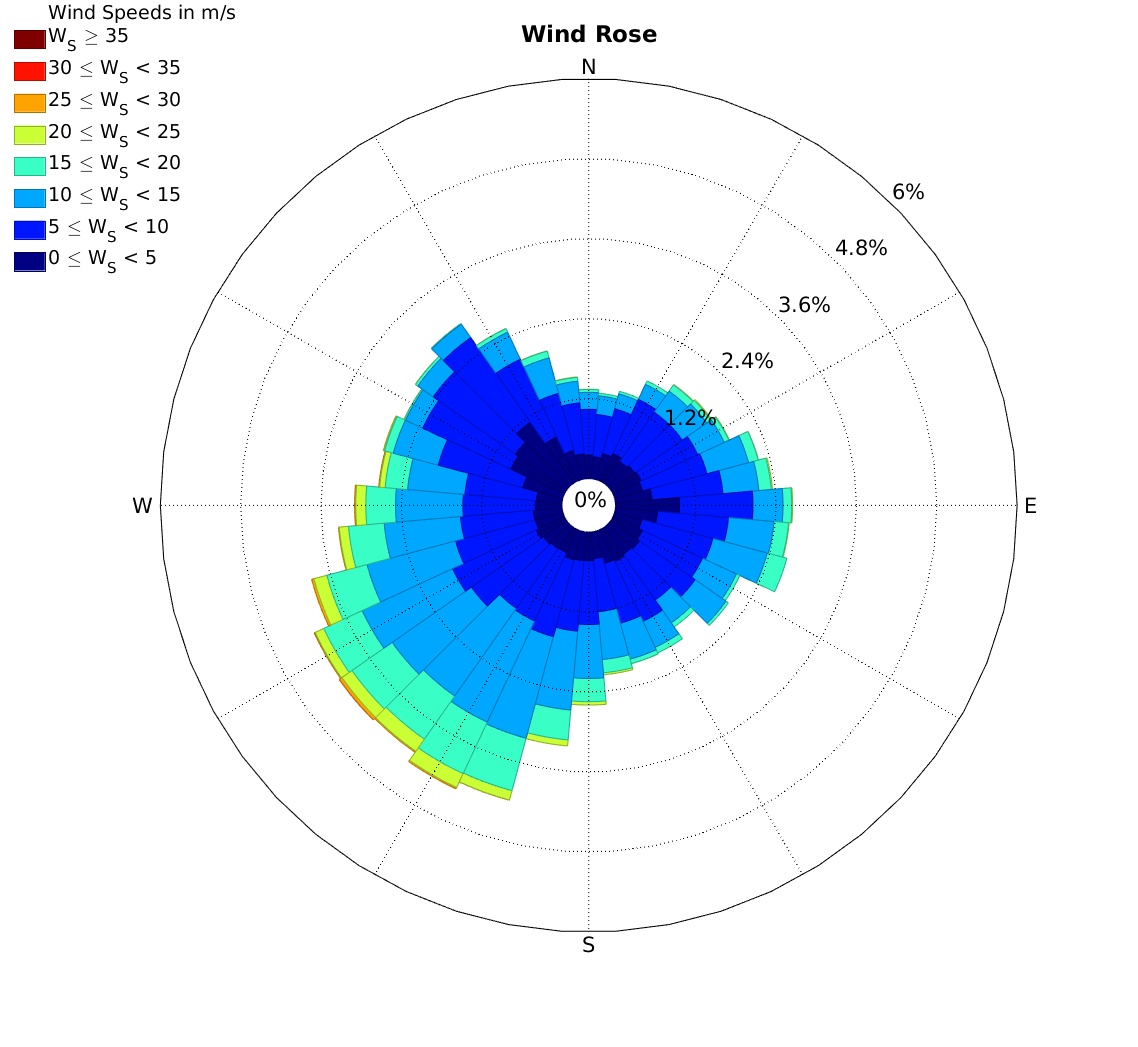
\includegraphics[width=1\linewidth]{../figures/WindRose_Fino1.png}
  \caption{Wind rose of FINO 1}
  \label{fig:Windrose_Fino1}
\end{subfigure}
\begin{subfigure}{0.5\textwidth}
  \centering
  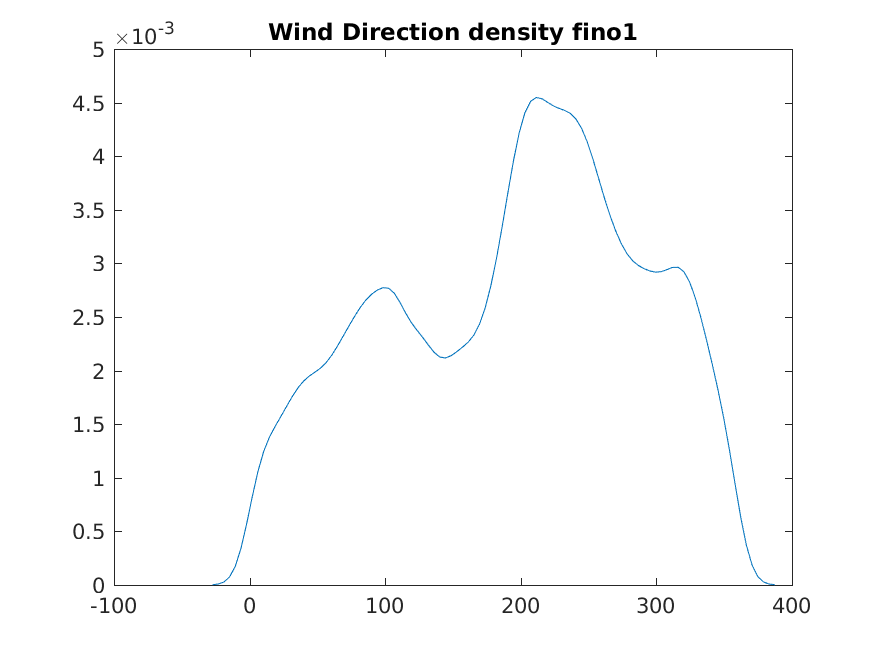
\includegraphics[width=1\linewidth]{../figures/Validation_WindRose_Fino1.png}
  \caption{pdf plot FINO 1}
    \label{fig:Windrose_Fino2}
\end{subfigure}
\end{figure}
\newpage
The pdf plot confirms that most of the wind is coming from south-west direction. This is identical with our FINO 1 wind rose. The same approach was used to confirm the wind rose created from FINO 2. (see Appendix)
After validating our results we now can compare the two windroses. See 

\begin{figure}[htb!]
\label{fig:WindRose1_valdidation}
\begin{subfigure}{0.5\textwidth}
  \centering
  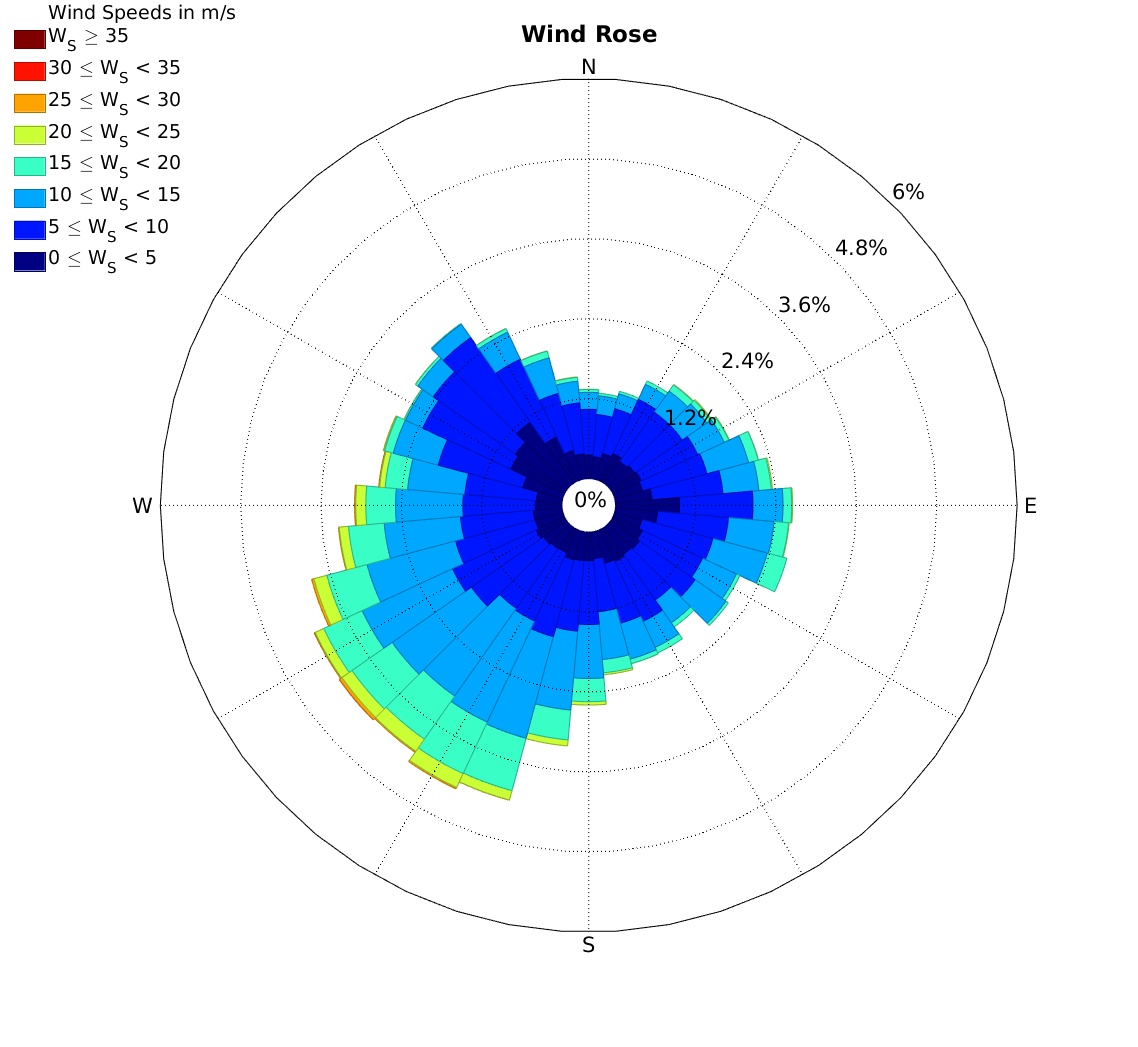
\includegraphics[width=1\linewidth]{../figures/WindRose_Fino1.png}
  \caption{Wind rose of FINO 1}
  \label{fig:Windrose_Fino1}
\end{subfigure}
\begin{subfigure}{0.5\textwidth}
  \centering
  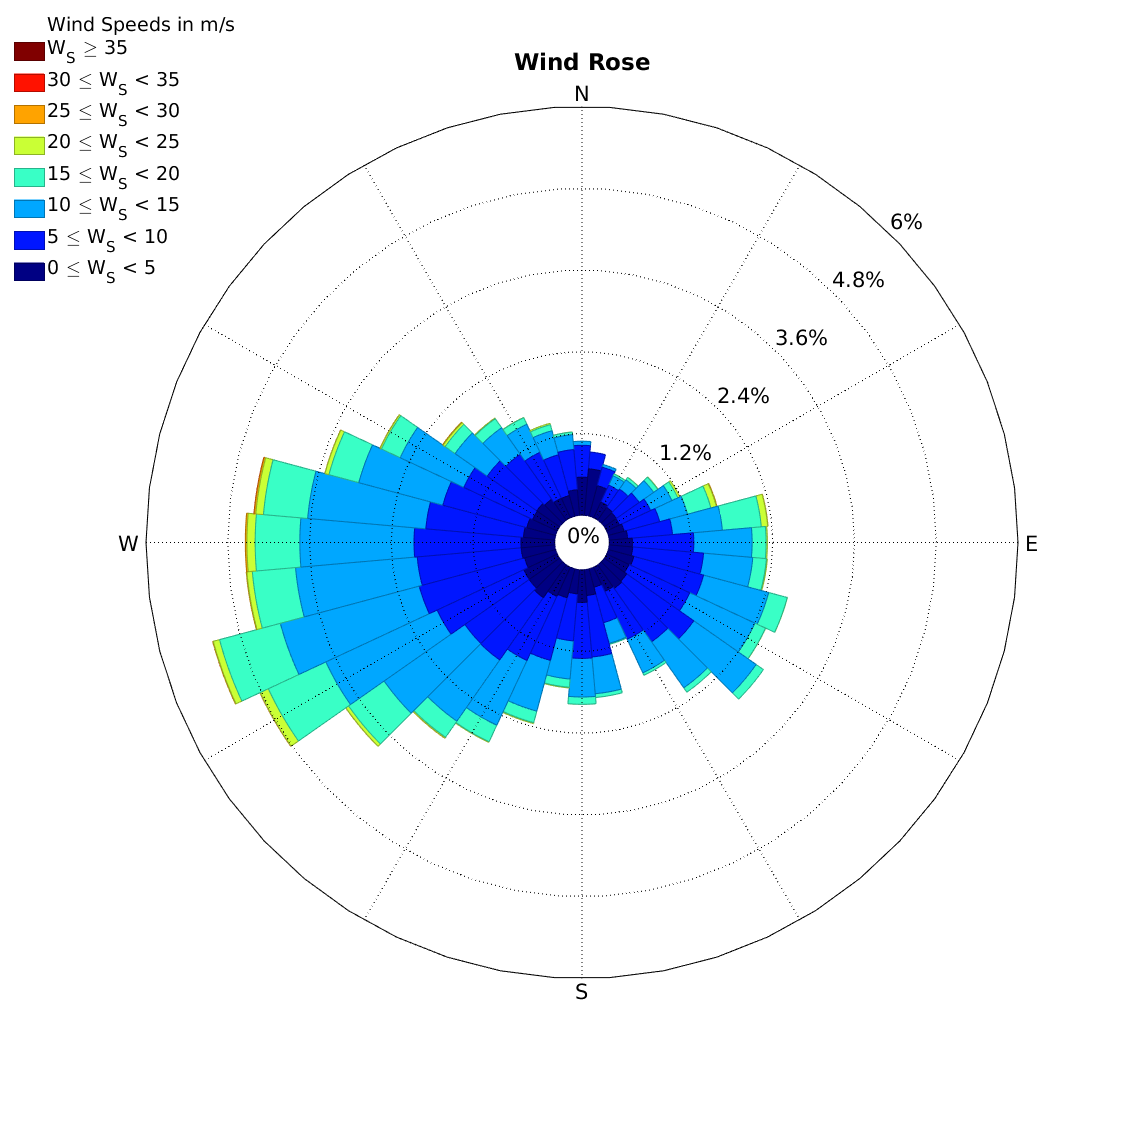
\includegraphics[width=1\linewidth]{../figures/WindRose_Fino2.png}
  \caption{Wind rose of FINO 2}
    \label{fig:Windrose_Fino2}
\end{subfigure}
\end{figure}
We observe that most of the the measured wind directions at FINO 1 are of south-western direction. For FINO 2, located in the baltic sea, the the wind is less distributed and has almost exclusively western and eastern directions. The difference in wind directions might be due to different pressure fields in the north sea and Baltic sea. Both met mast are located in the Northern Hemisphere. That means high pressure fields rotate clockwise and low pressure fields anti-clockwise. The wind directions are influenced by the isobars of the different pressure fields. Keeping this information in mind and looking at the content provided during the lecture (see. fig warm air advection), we can would the expect that the wind directions in the north sea have a south-west component. This coincides with our measured data. For FINO 2 we'd expect more or less only west and east components. This statement holds also for our measured data.
Both measurement systems are located in the open sea, so in general there are no obstacles that can create additional turbulence. However the construction of wind farms may influence the measurement.
\newpage
\section{Weighbull distribution}
In Task 2 we created histograms at around $90m$ height. Next we we calculated the weibull parameters, with the mean and standard deviation of the measured wind speeds. For the further calculation we used the equations provided during the lecture. We implemented the functions in Matlab and solved for the weibull parameters A and k. With the calculated parameters we created our weibull distribution.


\begin{lstlisting}
%% Task 2
mean1 = nanmean(fino1_v90);
dev1 = nanstd(fino1_v90);

mean2 = nanmean(fino2_v92);
dev2 = nanstd(fino2_v92);

% interpolate
k_Fino1 = 1;
Func_Fino1 = @(k_Fino1) (mean1*mean1/(dev1*dev1))*((gamma(1+2/k_Fino1))/(gamma(1+1/k_Fino1))^2-1)-1 
k_Fino1 = fsolve(Func_Fino1,k_Fino1);
disp(k_Fino1);
A_Fino1 = mean1/gamma(1+1/k_Fino1);
weibull_Fino1 = wblpdf(1:30,A_Fino1,k_Fino1);

k_Fino2 = 1;
Func_Fino2 = @(k_Fino2) (mean2*mean2/(dev2*dev2))*((gamma(1+2/k_Fino2))/(gamma(1+1/k_Fino2))^2-1)-1 
k_Fino2 = fsolve(Func_Fino2,k_Fino2);
disp(k_Fino2);
A_Fino2 = mean2/gamma(1+1/k_Fino2);
weibull_Fino2 = wblpdf(1:30,A_Fino2,k_Fino2);
\end{lstlisting}

Figure shows the histogram for Fino 1 and Fino 2 with the corresponding weibull fit.
\begin{figure}[htb!]
\label{fig:WindRose1_valdidation}
\begin{subfigure}{0.5\textwidth}
  \centering
  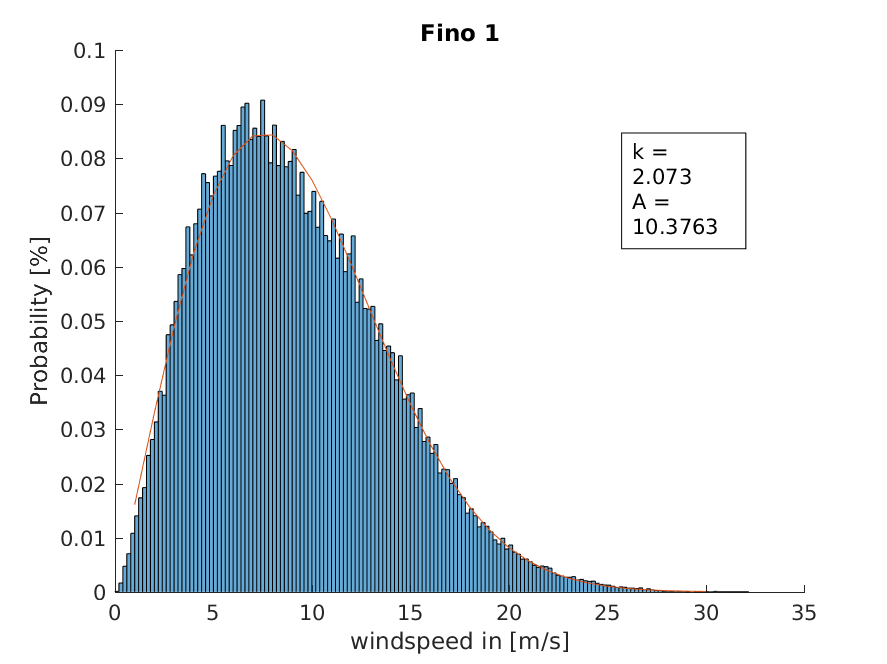
\includegraphics[width=1\linewidth]{../figures/Hist_withfit_Fino1.png}
  \caption{Histogram with weibull fit FINO 1}
  \label{fig:Windrose_Fino1}
\end{subfigure}
\begin{subfigure}{0.5\textwidth}
  \centering
  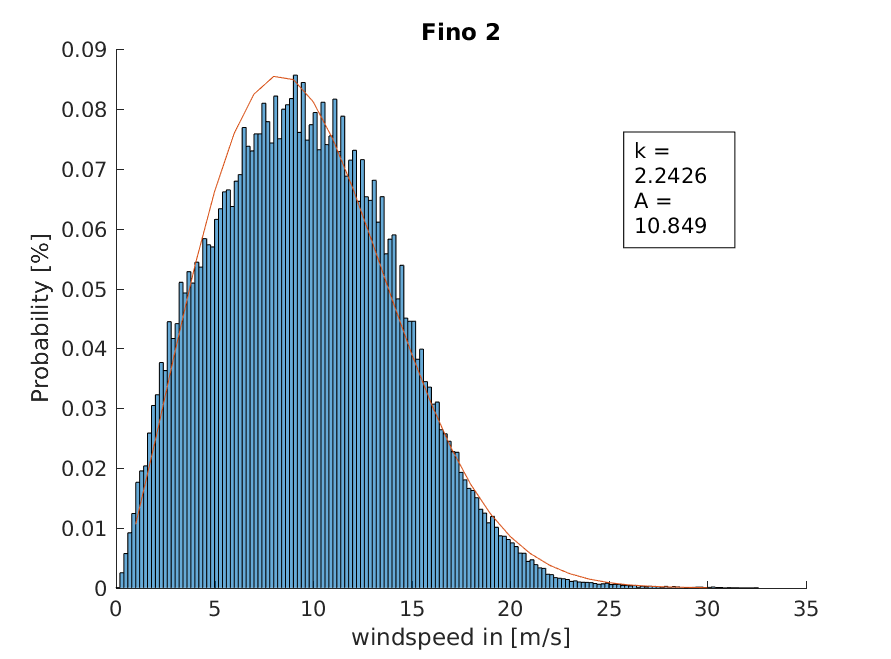
\includegraphics[width=1\linewidth]{../figures/Hist_withfit_Fino2.png}
  \caption{Histogram with weibull fit FINO 2}
    \label{fig:Windrose_Fino2}
\end{subfigure}
\end{figure}
In order to evaluate which region is more favourable for wind power utilization, we implemented two wind turbine power curves and calculated the energy yield.
The location of FINO 2 seems to be better for wind power utilization. This goes in hand with our first impression, because the curve of FINO 1 is more located at the left hand side.

\section{Vertical wind profiles}

\end{document}